\section{Performances of the Logistic Regression}
	In this section, when we describe the effect of each feature on the estimation of the risk of defaulting, we are dealing with the features specified in section \ref{sec:feature_engi}.\\

	By using all the features we considered in section \ref{sec:feature_engi}, we obtained an average log loss on the five folds of 0.66. Let's see the influence of each feature.

	\subsection{Impact of the 'salary' feature}
		This is our only numerical feature and we were very surprised to notice that it make a very big difference in the estimation of the risk but not in the good way. In fact, without it the average log loss on the five folds drops from 0.66 to 0.56. So we rejected it (also for the rest of the evaluation section).

	\subsection{Impact of the latent features}
		The latent features produced by the Latent Dirichlet Allocation based on the textual project description make the area under the ROC curve improves. But we observed thanks to the area under the ROC curve that even if the area is better, the classifier becomes less robust. In fact we noticed on the area under the ROC curve that the classifiers built during the cross validation had an area under the ROC curve less similar and close, and more irregular.
		On top of that, the average log loss on the five folds drop from 0.56 to 0.55 without them, so 1\% better. This goes in the same way as the irregularity of the area under the ROC curve.\\

		We took the decision to throw them away (also for the rest of the evaluation section) because even if the area under the ROC curve is better, that does not correspond to our problem setting which consist to estimate the risk of default. You can see in figure \ref{fig:auc_latent} the area under the ROC curve with and without the latent features.
		\begin{figure}[h!]
            \centering
            \begin{subfigure}[b]{0.98\textwidth}
                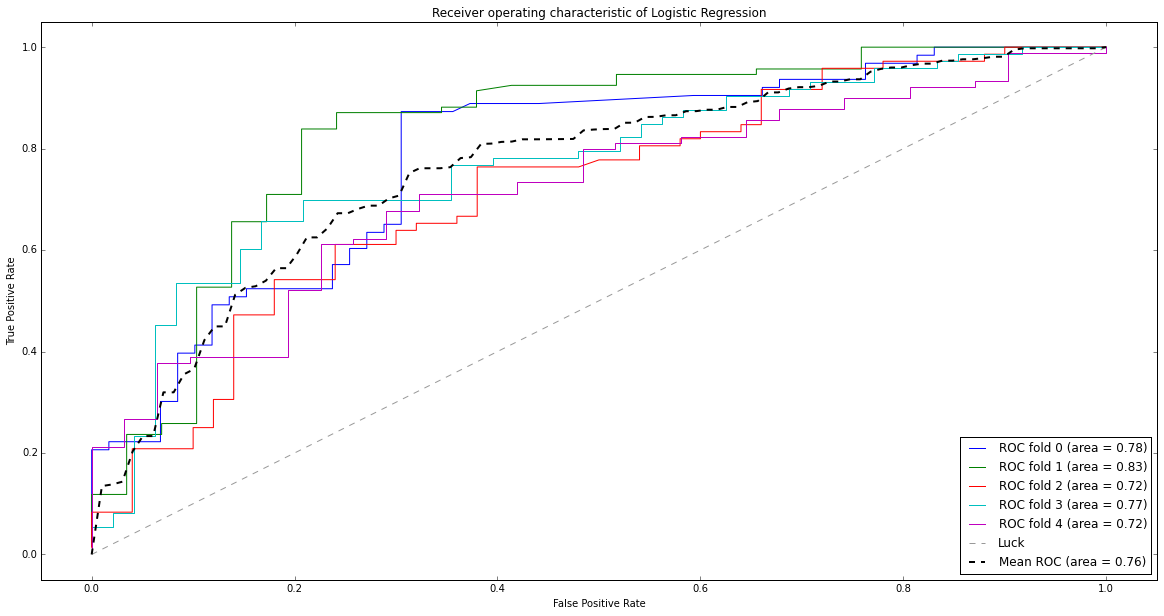
\includegraphics[width=\textwidth]{images/auc_without_latent.png}
                \caption{area under the ROC curve without the latent features.}
                \label{fig:auc_without_latent}
            \end{subfigure}
            \begin{subfigure}[b]{0.98\textwidth}
                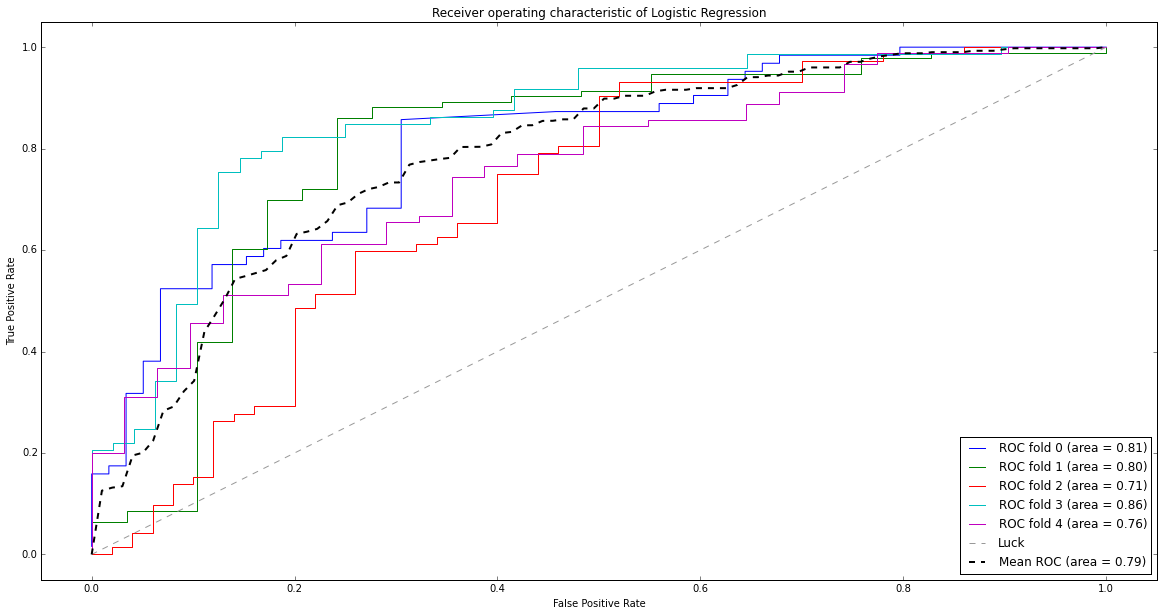
\includegraphics[width=\textwidth]{images/auc_with_latent.png}
                \caption{area under the ROC curve with the latent features.}
                \label{fig:auc_with_latent}
            \end{subfigure}
            \caption{Difference of area under the ROC curve with or without the latent features.}
            \label{fig:auc_latent}
        \end{figure}

	\subsection{Impact of the time feature}
		The time feature built based on the publication date of the loan really help the classifier. In fact the log loss increase from 0.55 to 0.59 without it. We explain that with the idea of context. In fact the contextual information brought by this feature informs of the economic situation and helps the estimation of the risk which is related to the economic situation. There may be more defaulting in certain periods of time than others.\\

		This kind of lending platform, like Bitbond, were born with the arrival of the currency Bitcoin. Moreover this currency were very popular during the Greek crisis for instance when all bank were closed. The popularity aspect implies an more important use of those platforms and if there are more use there is a higher probability of defaulting among the borrowers.\\

		This feature is kept for the estimation of the risk.

	\subsection{Impact of the Linear Discriminant Analysis}
		The Linear Discriminant Analysis done to reduce the dataset dimension before building the logistic regression model, has no impact on the log loss computation which is obviously normal since it is a linear model like the logistic regression. The only utility is when we build a SVM model that compute probability for each class, because the probability computation includes a five folds cross validation (for more detail see subsection \ref{ssec:svm}).

\section{Performances of the SVM}
	The performances of the SVM are basically the same. This due to the fact that both model are based on the same library (liblinear). We obtain like with logistic regression model a log loss of 0.55 with the same features and with or without the Linear Discriminant Analysis. This last one just makes the computation of the model faster : 2 minutes and 30 seconds without it and 3 seconds with.

\section{Hyperparameter setting}
	To set the hyperparameter we tried to use the \href{http://scikit-learn.org/stable/modules/generated/sklearn.grid_search.GridSearchCV.html#sklearn.grid_search.GridSearchCV}{GridSearchCV} of \textit{scikit-learn}. But after six hours it was still not done. That is why we chose to set it manually by trying different values for the C parameter of the \href{http://scikit-learn.org/stable/modules/generated/sklearn.linear_model.LogisticRegression.html#sklearn.linear_model.LogisticRegression}{LogisticRegression} by doing a nested five folds cross validation. We came to the conclusion that a $C=1$ was the best choice.